
\begin{abox}
	Practice Set-1
\end{abox}
\begin{enumerate}
	\item The $x$ - and $z$-components of a static magnetic field in a region are $B_{x}=B_{0}\left(x^{2}-y^{2}\right)$ and $B_{z}=0$, respectively. Which of the following solutions for its $y$-component is consistent with the Maxwell equations?
	{\exyear{ NET/JRF-(JUNE-2016)}}
	\begin{tasks}(2)
		\task[\textbf{a.}]$B_{y}=B_{0} x y$
		\task[\textbf{b.}]$B_{y}=-2 B_{0} x y$
		\task[\textbf{c.}] $B_{y}=-B_{0}\left(x^{2}-y^{2}\right)$
		\task[\textbf{d.}]  $B_{y}=B_{0}\left(\frac{1}{3} x^{3}-x y^{2}\right)$
	\end{tasks}
\begin{answer}
	\begin{align*}
	B_{x}&=B_{0}\left(x^{2}-y^{2}\right), B_{z}=0\\
	\because \vec{\nabla} \cdot \vec{B}&=0 \Rightarrow \frac{\partial B_{x}}{\partial x}+\frac{\partial B_{y}}{\partial y}+\frac{\partial B_{z}}{\partial z}=0 \Rightarrow \frac{\partial B_{y}}{\partial y}\\&=-\frac{\partial B_{x}}{\partial x}=-2 B_{0} x \Rightarrow B_{y}=-2 B_{0} x y
	\end{align*}
	So the correct answer is \textbf{Option (b)}
\end{answer}
	\item A current $i_{p}$ flows through the primary coil of a transformer. The graph of $i_{p}(t)$ as a function of time $t$ is shown in the figure below.\\
	\begin{figure}[H]
		\centering
		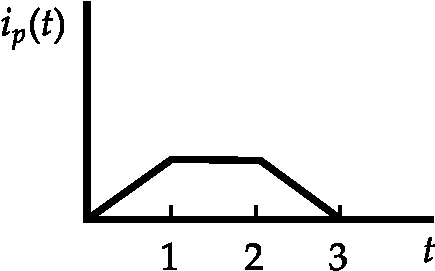
\includegraphics[height=3cm,width=4cm]{diagram-20211011(27)-crop}
	\end{figure}
	Which of the following graphs represents the current $i_{S}$ in the secondary coil?
	{\exyear{NET/JRF(JUNE-2014)}}
	\begin{tasks}(2)
		\task[\textbf{a.}] \begin{figure}[H]
			\centering
			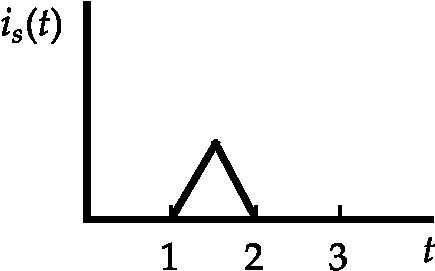
\includegraphics[height=3cm,width=4cm]{diagram-20211011(28)-crop}
		\end{figure}
		\task[\textbf{b.}] \begin{figure}[H]
			\centering
			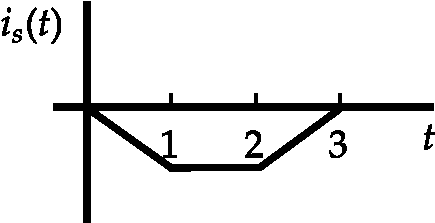
\includegraphics[height=3cm,width=4cm]{diagram-20211011(29)-crop}
		\end{figure}
		\task[\textbf{c.}] \begin{figure}[H]
			\centering
			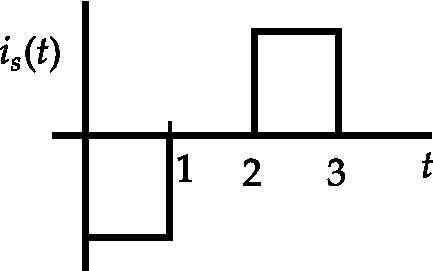
\includegraphics[height=3cm,width=4cm]{diagram-20211011(30)-crop}
		\end{figure}
		\task[\textbf{d.}] \begin{figure}[H]
			\centering
			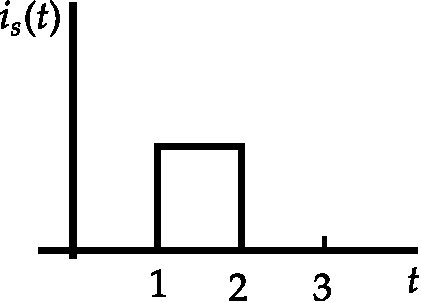
\includegraphics[height=3cm,width=4cm]{diagram-20211011(31)-crop}
		\end{figure}
	\end{tasks}
\begin{answer}
	\begin{align*}
	i_{s} \propto-\frac{d i_{p}}{d t}
	\end{align*}
	So the correct answer is \textbf{Option (c)}
\end{answer}
	\item A circular conducting wire loop is placed close to a solenoid as shown in the figure bellow. Also shown is the current through the solenoid as a function of solenoid as a function of time.\\
	\begin{figure}[H]
		\centering
		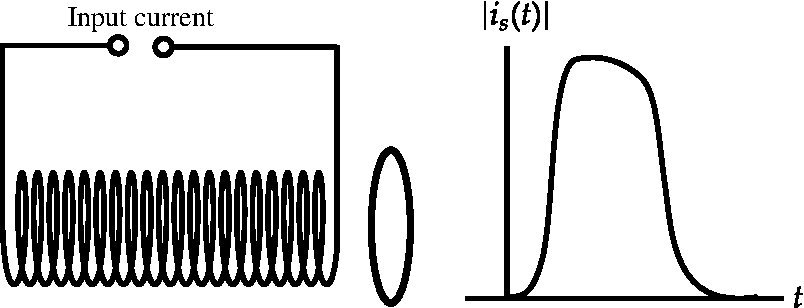
\includegraphics[height=3cm,width=8cm]{diagram-20211028(5)-crop}
	\end{figure}
	The magnitude $|i(t)|$ of the induced current in the wire loop, as a function of time $t$, is best represented as.
	{\exyear{NET/JRF(DEC-2019)}}
	\begin{tasks}(2)
		\task[\textbf{a.}] \begin{figure}[H]
			\centering
			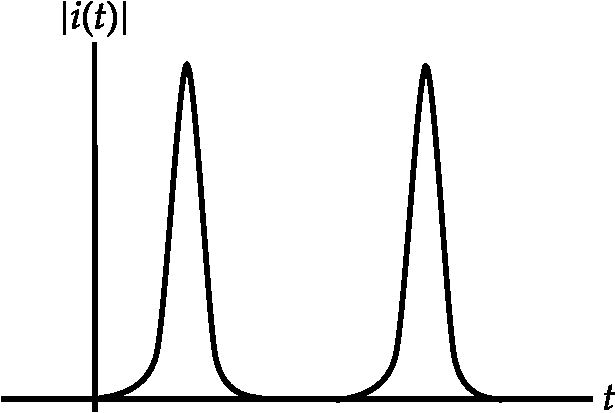
\includegraphics[height=3cm,width=5cm]{diagram-20211028(6)-crop}
		\end{figure}
		\task[\textbf{b.}] \begin{figure}[H]
			\centering
			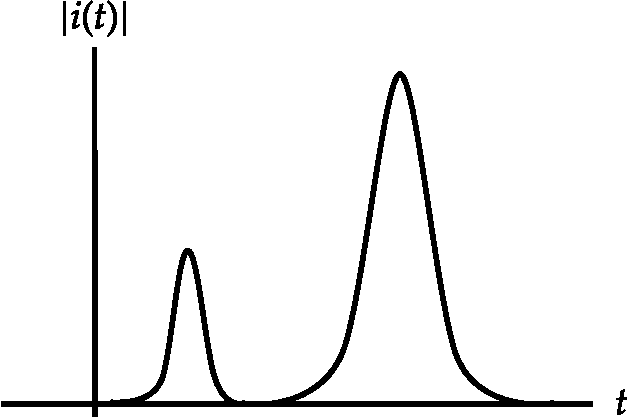
\includegraphics[height=3cm,width=5cm]{diagram-20211028(7)-crop}
		\end{figure}
		\task[\textbf{c.}] \begin{figure}[H]
			\centering
			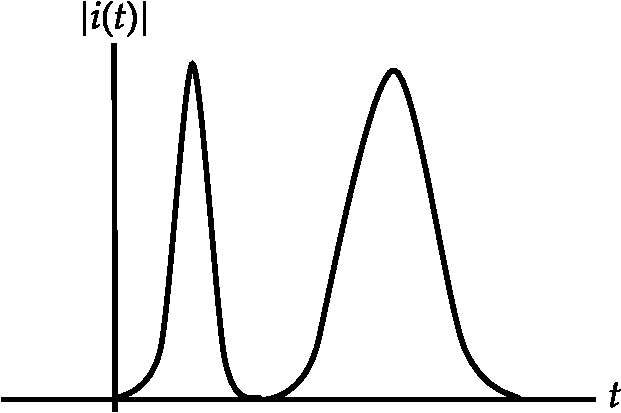
\includegraphics[height=3cm,width=5cm]{diagram-20211028(8)-crop}
		\end{figure}
		\task[\textbf{d.}] \begin{figure}[H]
			\centering
			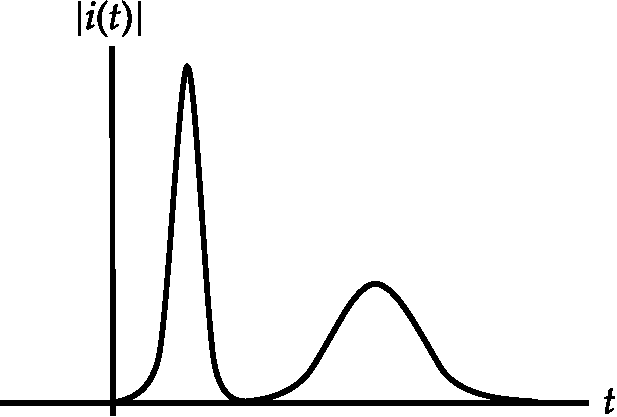
\includegraphics[height=3cm,width=5cm]{diagram-20211028(9)-crop}
		\end{figure}
	\end{tasks}
\begin{answer}
	\begin{align*}
	\text{	Induced e.m.f }\varepsilon& =-\frac{d \phi}{d t}, \quad|l(t)|=\frac{|\varepsilon|}{R} \propto\left|\frac{d l s}{d t}\right|
	\intertext{So when current increases,$|I(t)|$  will increase and when it will decrease $|I(t)|$ will
		decrease.}
	\end{align*}
	So the correct answer is \textbf{Option (d)}
\end{answer}
	\item A horizontal metal disc rotates about the vertical axis in a uniform magnetic field pointing up as shown in the figure. A circuit is made by connecting one end A of a resistor to the centre of the disc and the other end $B$ to its edge through a sliding contact. The current that flows through the resistor is
	{\exyear{NET/JRF(DEC-2013)}}
	\begin{figure}[H]
		\centering
		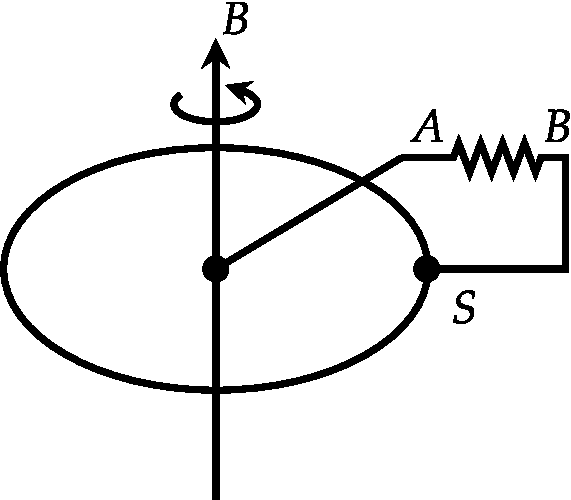
\includegraphics[height=4cm,width=5cm]{diagram-20211011(22)-crop}
	\end{figure}
	\begin{tasks}(4)
		\task[\textbf{a.}] Zero
		\task[\textbf{b.}] $D C$ from $A$ to $B$
		\task[\textbf{c.}] $D C$ from $B$ to $A$
		\task[\textbf{d.}] $A C$,
	\end{tasks}
\begin{answer}
	So the correct answer is \textbf{Option (b)}
\end{answer}
	\item  A conducting circular disc of radius $r$ and resistivity $\rho$ rotates with an angular velocity $\omega$ in a magnetic field $B$ perpendicular to it. A voltmeter is connected as shown in the figure below. Assuming its internal resistance to be infinite, the reading on the voltmeter
	{\exyear{NET/JRF(DEC-2016)}}
	\begin{figure}[H]
		\centering
		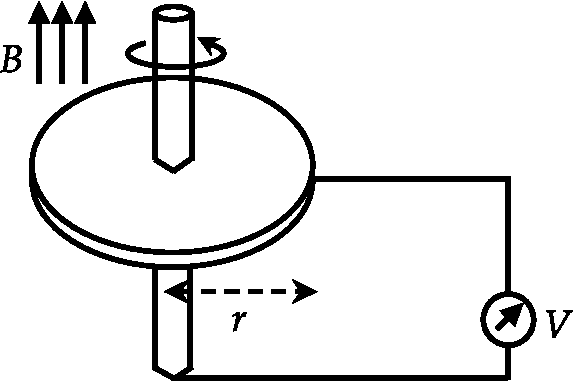
\includegraphics[height=3cm,width=5cm]{diagram-20211011(46)-crop}
	\end{figure}
	\begin{tasks}(1)
		\task[\textbf{a.}] Depends on $\omega, B, r$ and $\rho$
		\task[\textbf{b.}] Depends on $\omega, B$ and $r$ but not on $\rho$
		\task[\textbf{c.}]  Is zero because the flux through the loop is not changing
		\task[\textbf{d.}] Is zero because a current the flows in the direction of $B$
	\end{tasks}	
\begin{answer}
	\begin{align*}
	\text{Force }&\text{experienced by charge is}\\
	\vec{F}&=q(\vec{v} \times \vec{B})\text{ and }v=r \omega
	\end{align*}
	So the correct answer is \textbf{Option (b)}
\end{answer}
	\item A uniform magnetic field in the positive $z$-direction passes through a circular wire loop of radius $1 \mathrm{~cm}$ and resistance $1 \Omega$ lying in the $x y$-plane. The field strength is reduced from 10 tesla to 9 tesla in $1 s$. The charge transferred across any point in the wire is approximately
	{\exyear{ NET/JRF-(JUNE-2015)	}}
	\begin{tasks}(2)
		\task[\textbf{a.}] $3.1 \times 10^{-4}$ coulomb
		\task[\textbf{b.}]$3.4 \times 10^{-4}$ coulomb
		\task[\textbf{c.}]$4.2 \times 10^{-4}$ coulomb
		\task[\textbf{d.}] $5.2 \times 10^{-4}$ coulomb
	\end{tasks}	
\begin{answer}
	\begin{align*}
	\varepsilon&=-\frac{d \phi}{d t} \Rightarrow I=\frac{d q}{d t}=\frac{\varepsilon}{R}\\&=-\frac{1}{R} \frac{d \phi}{d t} \Rightarrow d q=-\frac{A}{R} d B=\frac{-\pi r^{2}}{R} d B\\
	\Rightarrow d q&=\frac{-3.14 \times\left(10^{-2}\right)^{2}}{1} \times 1=3.14 \times 10^{-4}\text{ coulomb}
	\end{align*}
	So the correct answer is \textbf{Option (a)}
\end{answer}
	\item A magnetic field $B$ is $B \hat{z}$ in the region $x>0$ and zero elsewhere. A rectangular loop, in the $x y$-plane, of sides $l$ (along the $x$-direction) and $h$ (along the $y$-direction) is inserted into the $x>0$ region from the $x<0$ region at constant velocity $v=v \hat{x}$. Which of the following values of $l$ and $h$ will generate the largest EMF?
	{\exyear{ NET/JRF-(JUNE-2016)	}}
	\begin{tasks}(2)
		\task[\textbf{a.}] $l=8, h=3$
		\task[\textbf{b.}]$l=4, h=6$
		\task[\textbf{c.}]$l=6, h=4$
		\task[\textbf{d.}]  $l=12, h=2$
	\end{tasks}	
\begin{answer}$\left. \right. $
	\begin{figure}[H]
		\centering
		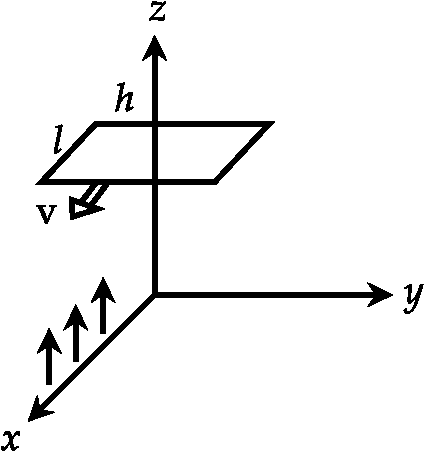
\includegraphics[height=4cm,width=5cm]{diagram-20211011(42)-crop}
	\end{figure}
	\begin{align*}
	\phi_{m} \propto B h x\\
	\varepsilon \propto \frac{-d \phi_{m}}{d t} \propto B v h \propto h
	\end{align*}
	So the correct answer is \textbf{Option (b)}
\end{answer}
	\item Consider a solenoid of radius $R$ with $n$ turns per unit length, in which a time dependent current $I=I_{0} \sin \omega t$ (where $\omega R / c<<1$ ) flows. The magnitude of the electric field at a perpendicular distance $r<R$ from the axis of symmetry of the solenoid, is
	{\exyear{NET/JRF-(DEC-2011)	}}
	\begin{tasks}(2)
		\task[\textbf{a.}]0
		\task[\textbf{b.}]$\frac{1}{2 r} \omega \mu_{0} n I_{0} R^{2} \cos \omega t$
		\task[\textbf{c.}]$\frac{1}{2} \omega \mu_{0} n I_{0} r \sin \omega t$
		\task[\textbf{d.}]  $\frac{1}{2} \omega \mu_{0} n I_{0} r \cos \omega t$
	\end{tasks}
\begin{answer}
	\begin{align*}
	\oint \vec{E} \cdot d \vec{l}&=-\int \frac{\partial \bar{B}}{\partial t} \cdot d \bar{a} ; \quad\left(\vec{B}=\mu_{0} n I(t) \hat{z}\right)\\
	\Rightarrow|\vec{E}| \times 2 \pi r&=-\mu_{0} n \frac{d I}{d t} \int_{r^{\prime}=0}^{r} 2 \pi r^{\prime} d r^{\prime}\\&=-\mu_{0} n \times I_{0} \omega \cos \omega t \times \frac{2 \pi r^{2}}{2}\\
	\Rightarrow|\vec{E}|&=-\frac{1}{2} \times \omega \mu_{0} n I_{0} r \cos \omega t
	\end{align*}
	So the correct answer is \textbf{Option (d)}
\end{answer}	
	\item A parallel plate capacitor is formed by two circular conducting plates of radius a separated by a distance $d$, where $d \ll a$. It is being slowly charged by a current that is nearly constant. At an instant when the current is $I$, the magnetic induction between the plates at a distance $\frac{a}{2}$ from the centre of the plate, is
	{\exyear{ NET/JRF-(DEC-2016)}}	
	\begin{tasks}(4)
		\task[\textbf{a.}]$\frac{\mu_{0} I}{\pi a}$
		\task[\textbf{b.}]$\frac{\mu_{0} I}{2 \pi a}$
		\task[\textbf{c.}]$\frac{\mu_{0} I}{a}$
		\task[\textbf{d.}]  $\frac{\mu_{0} I}{4 \pi a}$
	\end{tasks}	
\begin{answer}$\left. \right. $
	\begin{figure}[H]
		\centering
		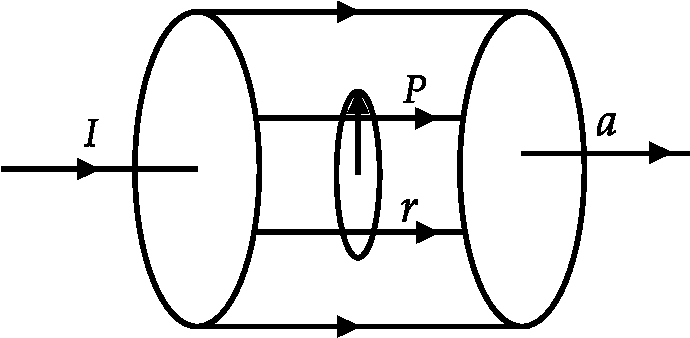
\includegraphics[height=2cm,width=5.5cm]{diagram-20211011(49)-crop}
	\end{figure}
	\begin{align*}
	|\vec{B}|&=\frac{\mu_{0} I r}{2 \pi a^{2}}\\
	|\vec{B}|&=\frac{\mu_{0} I}{4 \pi a}\text{ at }r=\frac{a}{2}
	\end{align*}
	So the correct answer is \textbf{Option (d)}
\end{answer}
	\item Suppose the $y z$-plane forms a chargeless boundary between two media of permittivities $\epsilon_{\text {left }}$ and $\epsilon_{\text {right }}$ where $\epsilon_{\text {left }}: \epsilon_{\text {right }}=1: 2$, if the uniform electric field on the left is $\vec{E}_{\text {left }}=c(\hat{i}+\hat{j}+\hat{k})$ (where $c$ is a constant), then the electric field on the right $\vec{E}_{\text {right }}$ is
	{\exyear{NET/JRF(JUNE-2015)}}
	\begin{tasks}(4)
		\task[\textbf{a.}]  $c(2 \hat{i}+\hat{j}+\hat{k})$
		\task[\textbf{b.}] $c(\hat{i}+2 \hat{j}+2 \hat{k})$
		\task[\textbf{c.}] $c\left(\frac{1}{2} \hat{i}+\hat{j}+\hat{k}\right)$
		\task[\textbf{d.}] $c\left(\hat{i}+\frac{1}{2} \hat{j}+\frac{1}{2} \hat{k}\right)$
	\end{tasks}
\begin{answer}$\left. \right. $
	\begin{figure}[H]
		\centering
		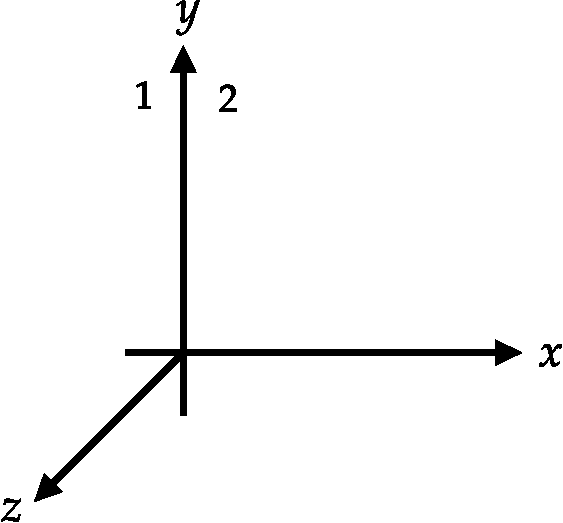
\includegraphics[height=4cm,width=4.5cm]{diagram-20211011(34)-crop}
	\end{figure}
	\begin{align*}
	E_{1}^{\prime \prime}&=c(\hat{j}+\hat{k})=E_{2}^{\prime \prime}\\
	D_{1}^{\perp}&=D_{2}^{\perp} \Rightarrow \epsilon_{1} E_{1}^{\perp}=\epsilon_{2} E_{2}^{\perp} \Rightarrow E_{2}^{1}=\frac{\epsilon_{1}}{\epsilon_{2}} E_{1}^{\perp}\\
	\Rightarrow E_{2}^{\perp}&=\frac{1}{2} c \hat{i} \Rightarrow \vec{E}_{2}=c\left(\frac{1}{2} \hat{i}+\hat{j}+\hat{k}\right)
	\end{align*}
	So the correct answer is \textbf{Option (c)}
\end{answer}
	\item  The half space region $x>0$ and $x<0$ are filled with dielectric media of dielectric constants $\varepsilon_{1}$ and $\varepsilon_{2}$ respectively. There is a uniform electric field in each part. In the right half, the electric field makes an angle $\theta_{1}$ to the interface. The corresponding angle $\theta_{2}$ in the left half satisfies
	{{\exyear{NET/JRF(JUNE-2016)}}}
	\begin{figure}[H]
		\centering
		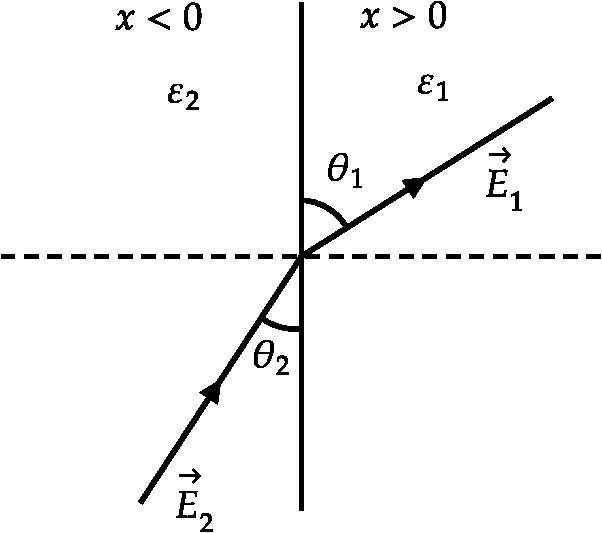
\includegraphics[height=4cm,width=4cm]{diagram-20211011(41)-crop}
	\end{figure}
	\begin{tasks}(2)
		\task[\textbf{a.}] $\varepsilon_{1} \sin \theta_{2}=\varepsilon_{2} \sin \theta_{1}$
		\task[\textbf{b.}] $\varepsilon_{1} \tan \theta_{2}=\varepsilon_{2} \tan \theta_{1}$
		\task[\textbf{c.}] $\varepsilon_{1} \tan \theta_{1}=\varepsilon_{2} \tan \theta_{2}$
		\task[\textbf{d.}] $\varepsilon_{1} \sin \theta_{1}=\varepsilon_{2} \sin \theta_{2}$
	\end{tasks}
\begin{answer}
	\begin{align*}
	\frac{\tan \theta_{1}}{\tan \theta_{2}}&=\frac{\frac{E_{1}^{\perp}}{E_{1}^{\|}}}{\frac{E_{2}^{\perp}}{E_{2}^{\|}}}=\frac{E_{1}^{\perp}}{E_{2}^{\perp}} \quad\left(\because E_{1}^{\|}=E_{2}^{\|}\right)\\
	D_{1}^{\perp}&=D_{2}^{\perp} \Rightarrow \varepsilon_{1} E_{1}^{\perp}=\varepsilon_{2} E_{2}^{\perp} \Rightarrow \frac{E_{1}^{\perp}}{E_{2}^{\perp}}=\frac{\varepsilon_{2}}{\varepsilon_{1}} \Rightarrow \frac{\tan \theta_{1}}{\tan \theta_{2}}\\&=\frac{\varepsilon_{2}}{\varepsilon_{1}} \Rightarrow \varepsilon_{1} \tan \theta_{1}=\varepsilon_{2} \tan \theta_{2}
	\end{align*}
	So the correct answer is \textbf{Option (c)}
\end{answer}
	\item Which of the following is not a correct boundary condition at an interface between two homogeneous dielectric media? (In the following $\hat{n}$is a unit vector normal to the  interface, $\sigma$ and $\vec{j}_s$, are the surface charge and current densities, respectively.)
	{\exyear{NET/JRF(JUNE-2019)}}
	\begin{tasks}(2)
		\task[\textbf{a.}] $\hat{n} \times\left(\vec{D}_{1}-\vec{D}_{2}\right)=0$
		\task[\textbf{b.}] $\hat{n} \times\left(\vec{H}_{1}-\vec{H}_{2}\right)=\vec{j}_{s}$
		\task[\textbf{c.}] $\hat{n} \cdot\left(\vec{D}_{1}-\vec{D}_{2}\right)=\sigma$
		\task[\textbf{d.}] $\hat{n} \cdot\left(\vec{B}_{1}-\vec{B}_{2}\right)=0$
	\end{tasks}
\begin{answer}
	\begin{align*}
	\intertext{Since media is homogeneous dielectric:
		assume uniform polarisation and
		magnetisation.}
	\intertext{$\sigma$ and $\vec{j }_s$ , are the free surface charge and free surface current densities.}
	\vec{\nabla} \times \vec{D}&=0 \quad \Rightarrow D_{1}^{\|}=D_{2}^{\|} \\ \because \vec{\nabla} \times \vec{P}&=0 \quad\text{ and }\quad D_{1}^{\perp}-D_{2}^{\perp}=\sigma\\
	\text{Thus }\left(\vec{D}_{1}-\vec{D}_{2}\right)&=\sigma \hat{n}\\
	\Rightarrow \hat{n} \cdot\left(\vec{D}_{1}-\vec{D}_{2}\right)&=\sigma \quad\text{ and } \hat{n} \times\left(\vec{D}_{1}-\vec{D}_{2}\right) \neq 0\\
	\vec{\nabla} \cdot \vec{H}&=-\vec{\nabla} \cdot \vec{M}=0 \quad \Rightarrow H_{1}^{\perp}=H_{2}^{\perp} \\ \because \vec{\nabla} \cdot \vec{M}&=0 \quad\text{ and } \quad H_{1}^{\|}-H_{2}^{\|}=j_{s}\\
	\text{	Thus }\left(\vec{H}_{1}-\vec{H}_{2}\right)=\vec{j}_{s} \times \hat{n}\\
	\Rightarrow \hat{n} \times\left(\vec{H}_{1}-\vec{H}_{2}\right)&=\vec{j}_{s}\\
	\text{Also}
	\intertext{$\vec{\nabla} \cdot \vec{B}=0 \quad \Rightarrow B_{1}^{\perp}=B_{2}^{\perp} \quad$ and $\quad B_{1}^{\|}-B_{1}^{\|}=\mu_{0} K$ (assume $K$ is total surface current at interface)}\\
	\text{Thus }\left(\vec{B}_{1}-\vec{B}_{2}\right)&=\mu_{0}(\vec{K} \times \hat{n}) .\\
	\Rightarrow \hat{n} \cdot\left(\vec{B}_{1}-\vec{B}_{2}\right)&=0
	\end{align*}
	So the correct answer is \textbf{Option (a)}
\end{answer}
\end{enumerate}
\colorlet{ocre1}{ocre!70!}
\colorlet{ocrel}{ocre!30!}
\setlength\arrayrulewidth{1pt}
\begin{table}[H]
	\centering
	\arrayrulecolor{ocre}
	\begin{tabular}{|p{1.5cm}|p{1.5cm}||p{1.5cm}|p{1.5cm}|}
		\hline
		\multicolumn{4}{|c|}{\textbf{Answer key}}\\\hline\hline
		\rowcolor{ocrel}Q.No.&Answer&Q.No.&Answer\\\hline
		1&\textbf{b} &2&\textbf{c}\\\hline 
		3&\textbf{d} &4&\textbf{c} \\\hline
		5&\textbf{b} &6&\textbf{a} \\\hline
		7&\textbf{b}&8&\textbf{d}\\\hline
		9&\textbf{d}&10&\textbf{c}\\\hline
		11&\textbf{c} &12&\textbf{a}\\\hline
		
	\end{tabular}
\end{table}
\newpage
\begin{abox}
	Practice Set-2
\end{abox}
\begin{enumerate}
	\item Two rails of a railroad track are insulated from each other and from the ground, and are connected by a millivoltmeter. What is the reading of the millivoltmeter when a train travels at the speed $90 \mathrm{~km} / \mathrm{hr}$ down the track? Assume that the vertical component of the earth's magnetic field is $0.2$ gauss and that the tracks are separated by two meters. Use 1 gauss $=10^{-4}$ Tesla $=10^{-4} \mathrm{~V} \cdot \mathrm{sec} / \mathrm{m}^{2}$
	{\exyear{ JEST-2020}}
	\begin{tasks}(4)
		\task[\textbf{a.}]10
		\task[\textbf{b.}]1
		\task[\textbf{c.}]$0.2$
		\task[\textbf{d.}]180 
	\end{tasks}
\begin{answer}
	\begin{align*}
	\text { Magnetic flux } \phi_{m}&=B l x \Rightarrow \text { e.m.f } \varepsilon=-\frac{d \phi_{m}}{d t}=-B l v\\
	\Rightarrow|\varepsilon|&=0.2 \times 10^{-4} \times 2 m \times \frac{90 \times 10^{3}}{3600} \text { Volts } \Rightarrow|\varepsilon|=1 \mathrm{mV}
	\end{align*}
		So the correct answer is \textbf{Option (b)}
\end{answer}
	\item 	Which of the following expressions represents an electric field due to a time varying magnetic field?
	{\exyear{ JEST-2015}}
	\begin{tasks}(2)
		\task[\textbf{a.}]$K(x \hat{x}+y \hat{y}+z \hat{z})$
		\task[\textbf{b.}] $K(x \hat{x}+y \hat{y}-z \hat{z})$
		\task[\textbf{c.}]$K(x \hat{x}-y \hat{y})$
		\task[\textbf{d.}]$K(y \hat{y}-x \hat{y}+2 z \hat{z})$ 
	\end{tasks}	
\begin{answer}
	\begin{align*}
	\vec{B} \neq \vec{\nabla} \times \vec{A}\\
	\end{align*}
	So the correct answer is \textbf{Option (c)}
\end{answer}
	\item Two parallel rails of a railroad track are insulated from each other and from the ground. The distance between the rails is 1 meter. A voltmeter is electrically connected between the rails. Assume the vertical component of the earth's magnetic field to the $0.2$ gauss. What is the voltage developed between the rails when a train travels at a speed of $180 \mathrm{~km} / \mathrm{h}$ along the track? Give the answer in milli-volts.
	{\exyear{ JEST-2018}}
	\begin{answer}
		\begin{align*}
		\text { Induced emf } \varepsilon=B l v=\left(0.2 \times 10^{-4}\right) \times 1 \mathrm{~m} \times 180 \times \frac{10}{60 \times 60}=10^{-3} \text { volts }=1 \mathrm{mV}
		\end{align*}
			So the correct answer is \textbf{1.0}
	\end{answer}
	\item 	A very long solenoid (axis along $z$ direction) of $n$ turns per unit length carries a current which increases linearly with time, $i=K t$. What is the magnetic field inside the solenoid at a given time $t$ ?
	{\exyear{ JEST-2019}}
	\begin{tasks}(2)
		\task[\textbf{a.}]$\vec{B}=\mu_{0} n K t \hat{z}$
		\task[\textbf{b.}]$\vec{B}=\mu_{0} n K \hat{z}$
		\task[\textbf{c.}]$\vec{B}=\mu_{0} n K t(\hat{x}+\hat{y})$
		\task[\textbf{d.}] $\vec{B}=\mu_{0} c n K t \hat{z}$
	\end{tasks}	
\begin{answer}
	So the correct answer is \textbf{Option (a)}
\end{answer}
	\item 	A circular metal loop of radius $a=1 \mathrm{~m}$ spins with a constant angular velocity $\omega=20 \pi \mathrm{rad} / \mathrm{s}$ in a magnetic field $B=3$ Tesla, as shown in the figure. The resistance of the loop is 10 ohms. Let $P$ be the power dissipated in one complete cycle. What is the value of $\frac{P}{\pi^{4}}$ in Watts?
	{\exyear{ JEST-2019}}
	\begin{figure}[H]
		\centering
		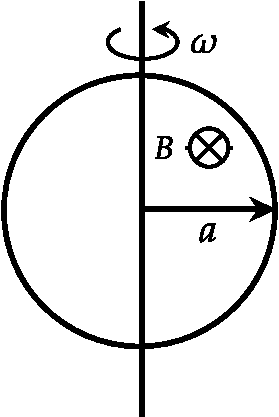
\includegraphics[height=4cm,width=2.8cm]{ED-20}
	\end{figure}
\begin{answer}
	\begin{align*}
	\text { Magnetic flux through the loop is } \phi_{m}&=\int_{S} \vec{B} d \vec{a}=B \times \pi a^{2} \times \cos \omega t\\
	\text { Induced e.m.f } \varepsilon&=-\frac{d \phi_{m}}{d t}=\omega B \times \pi a^{2} \times \sin \omega t\\
	Power dissipated
	p=\frac{\varepsilon^{2}}{R}&=\frac{\omega^{2} B^{2} \pi^{2} a^{4} \sin ^{2} \omega t}{R}\\
	\text{Power dissipated in one complete cycle }P&=\langle p\rangle=\frac{\omega^{2} B^{2} \pi^{2} a^{4}}{2 R}
	\because\left\langle\sin ^{2} \omega t\right\rangle=\frac{1}{2}\\
	\frac{P}{\pi^{4}}&=\frac{\omega^{2} B^{2} a^{4}}{2 \pi^{2} R} \Rightarrow P=\frac{(20 \pi)^{2}(3)^{2}(1)^{4}}{2(10)(10)}=18
	\end{align*}
		So the correct answer is \textbf{18}
\end{answer}
	\item Self inductance per unit length of a long solenoid of radius $R$ with $n$ turns per unit length is:
	{\exyear{ JEST-2016}}
	\begin{tasks}(4)
		\task[\textbf{a.}]$\mu_{0} \pi R^{2} n^{2}$
		\task[\textbf{b.}]$2 \mu_{0} \pi R^{2} n$
		\task[\textbf{c.}]$2 \mu_{0} \pi R^{2} n^{2}$
		\task[\textbf{d.}] $\mu_{0} \pi R^{2} n$
	\end{tasks}	
\begin{answer}
	So the correct answer is \textbf{Option (a)}
\end{answer}
	\item The $x-y$ plane is the boundary between free space and a magnetic material with relative permeability $\mu_{r}$. The magnetic field in the free space is $B_{x} \hat{i}+B_{z} \hat{k}$. The magnetic field in the magnetic material is
	{\exyear{ GATE- 2016}}
	\begin{tasks}(2)
		\task[\textbf{a.}]$B_{x} \hat{i}+B_{z} \hat{k}$
		\task[\textbf{b.}]$B_{x} \hat{i}+\mu_{r} B_{z} \hat{k}$
		\task[\textbf{c.}] $\frac{1}{\mu_{r}} B_{x} \hat{i}+B_{z} \hat{k}$
		\task[\textbf{d.}] $\mu_{r} B_{x} \hat{i}+B_{z} \hat{k}$
	\end{tasks}	
\begin{answer}
	\begin{align*}
	B_{1}^{\perp}&=B_{z} \hat{k}=B_{2}^{\perp}\text{ and }H_{1}^{\|}=\\&H_{2}^{\|} \Rightarrow \frac{B_{1}^{\|}}{\mu_{0}}=\frac{B_{2}^{\|}}{\mu_{0} \mu_{r}} \Rightarrow B_{2}^{\|}\\&=\mu_{r} B_{1}^{\|}=\mu_{r} B \hat{i}
	\intertext{The magnetic field in the magnetic material is $\mu_{r} B_{x} \hat{i}+B_{z} \hat{k}$}
	\end{align*}
	So the correct answer is \textbf{Option (d)}
\end{answer}
	\item 	At a surface current, which one of the magnetostatic boundary condition is $\underline{\text { NOT }}$ CORRECT?
	{\exyear{ GATE- 2013}}
	\begin{tasks}(1)
		\task[\textbf{a.}]Normal component of the magnetic field is continuous.
		\task[\textbf{b.}]Normal component of the magnetic vector potential is continuous.
		\task[\textbf{c.}] Tangential component of the magnetic vector potential is continuous.
		\task[\textbf{d.}] Tangential component of the magnetic vector potential is not continuous.
	\end{tasks}
\begin{answer}
	So the correct answer is \textbf{Option (d)}
\end{answer}
	\item A circular loop made of a thin wire has radius $2 \mathrm{~cm}$ and resistance $2 \Omega$. It is placed perpendicular to a uniform magnetic field of magnitude $\left|\vec{B}_{0}\right|=0.01$ Tesla. At time $t=0$ the field starts decaying as $\vec{B}=\vec{B}_{0} e^{-t / t_{0}}$, where $t_{0}=1 s$. The total charge that passes through a cross section of the wire during the decay is $Q$. The value of $Q$ in $\mu C$ (rounded off to two decimal places) is
	{\exyear{ GATE- 2019}}
	\begin{answer}
		\begin{align*}
		\varepsilon&=-\frac{d \phi}{d t}=-\frac{A d B}{d t}, I\\&=\frac{\varepsilon}{R}=-\frac{d \phi}{d t} \frac{1}{R}\\
		\Rightarrow-\frac{d \phi}{d t}&=-\pi r^{2} \frac{d}{d t}\left(B_{0} e^{-t / t_{0}}\right)\\&=\pi r^{2} B_{0} e^{-t}\left(t_{0}=1\right)\\
		Q&=\int_{0}^{\infty} I(t) d t=\int_{0}^{\infty} \frac{\pi r^{2}}{R} B_{0} e^{-t} d t\\&=\frac{\pi r^{2} B_{0}}{R}\left|\frac{e^{-t}}{-1}\right|_{0}^{\infty}\\
		&=3.14 \times\left(2 \times 10^{-2}\right)^{2} \times 0.01\\&=6.28 \mu C
		\end{align*}
	\end{answer}
	\item A long solenoid is embedded in a conducting medium and is insulated from the medium. If the current through the solenoid is increased at a constant rate, the induced current in the medium as a function of the radial distance $r$ from the axis of the solenoid is proportional to
	{\exyear{GATE- 2015}}
	\begin{tasks}(1)
		\task[\textbf{a.}] $r^{2}$ inside the solenoid and $\frac{1}{r}$ outside
		\task[\textbf{b.}]$r$ inside the solenoid and $\frac{1}{r^{2}}$ outside
		\task[\textbf{c.}]$r^{2}$ inside the solenoid and $\frac{1}{r^{2}}$ outside
		\task[\textbf{d.}] $r$ inside the solenoid and $\frac{1}{r}$ outside
	\end{tasks}
\begin{answer}
	\begin{align*}
	\oint \vec{E} \cdot d \vec{l}&=-\int \frac{\partial \vec{B}}{\partial t} \cdot d \vec{a}\\
	\text{	For }r<R,|\vec{E}| 2 \pi r&=-\mu_{0} n \frac{d I}{d t} \int_{r^{\prime}=0}^{r} 2 \pi r^{\prime} d r^{\prime}\\&=-\mu_{0} n \frac{d I}{d t} \frac{2 \pi r^{2}}{2} \Rightarrow|\vec{E}|\\&=-\frac{1}{2} \mu_{0} n \frac{d I}{d t} r\\
	\text{For }r>R,|\vec{E}| 2 \pi r&=-\mu_{0} n \frac{d I}{d t} \int_{r^{\prime}=0}^{R} 2 \pi r^{\prime} d r^{\prime}\\&=-\mu_{0} n \frac{d I}{d t} \frac{2 \pi R^{2}}{2} \Rightarrow|\vec{E}|\\&=-\frac{1}{2 r} \mu_{0} n \frac{d I}{d t} R^{2}
	\end{align*}
\end{answer}
	\item Consider an infinitely long solenoid with $N$ turns per unit length, radius $R$ and carrying a current $I(t)=\alpha \cos \omega t$, where $\alpha$ is a constant and $\omega$ is the angular frequency. The magnitude of electric field at the surface of the solenoid is
	\begin{tasks}(2)
		\task[\textbf{a.}]$\frac{1}{2} \mu_{0} N R \omega \alpha \sin \omega t$
		\task[\textbf{b.}]$\frac{1}{2} \mu_{0} \omega N R \cos \omega t$
		\task[\textbf{c.}]$\mu_{0} N R \omega \alpha \sin \omega t$
		\task[\textbf{d.}] $\mu_{0} \omega N R \cos \omega t$
	\end{tasks}
\begin{answer}
	\begin{align*}
	\vec{B}=\left\{\begin{array}{ll}\mu_{0} N I(t) \hat{z}, \text { inside } \\ 0 \quad \quad, \text { outside }\end{array}\right.\\
	\text{	Since, }\oint_{\text {line }} \vec{E} \cdot d \vec{l}&=-\int \frac{\partial \vec{B}}{\partial t} \cdot d \vec{a}\\
	\Rightarrow|\vec{E}| \times 2 \pi R&=-\mu_{0} N(-\alpha \omega \sin \omega t) \times \pi R^{2}\\
	\Rightarrow|\vec{E}|&=\frac{1}{2} \mu_{0} N R \omega \alpha \sin \omega t
	\end{align*}
	So the correct answer is \textbf{Option (a)}
\end{answer}
	\item A medium $\left(\varepsilon_{r}>1, \mu_{r}=1, \sigma>0\right)$ is semi-transparent to an electromagnetic wave when
	{\exyear{ GATE- 2020}}
	\begin{tasks}(1)
		\task[\textbf{a.}]Conduction current $\gg>$ Displacement current
		\task[\textbf{b.}]Conduction current $<<$ Displacement current
		\task[\textbf{c.}]Conduction current $=$ Displacement current
		\task[\textbf{d.}] Both Conduction current and Displacement current are zero
	\end{tasks}
\begin{answer}
	\begin{align*}
	\text { Conduction current } J_{c}&=\sigma E=\sigma E_{0} \cos \omega t\\
	\text { Displacement current } J_{d}&=\varepsilon \frac{\partial E}{\partial t} \Rightarrow\left|J_{d}\right|=\omega \varepsilon E_{0} \sin \omega t
	\intertext{For semi-transparent medium i.e for poor conductor $\sigma<<\omega \varepsilon$.}
	\text { Let } \omega t&=\frac{\pi}{4} \Rightarrow \frac{J_{c}}{J_{d}}=\frac{\sigma E_{0}}{\omega \varepsilon E_{0}}=\frac{\sigma}{\omega \varepsilon}<<1 \Rightarrow J_{c}<<J_{d}
	\end{align*}
		So the correct answer is \textbf{Option (b)}
\end{answer}
	\item A sinusoidal voltage of the form $V(t)=V_{0} \cos (\omega t)$ is applied across a parallel plate capacitor placed in vacuum. Ignoring the edge effects, the induced emf within the region between the capacitor plates can be expressed as a power series in $\omega$. The lowest nonvanishing exponent in $\omega$ is -----------
	{\exyear{ GATE- 2020}}
	\begin{answer}
		\begin{align*}
		\text { Induced e.m.f } \varepsilon&=-\frac{d \phi}{d t}=-\frac{A d B}{d t}\\
		\oint \vec{B} \cdot d \dot{l}&=\mu_{0} I_{\text {enc }}+\mu_{0} \varepsilon_{0} \int_{S} \frac{\partial \vec{E}}{\partial t} \cdot d \vec{a}
		\intertext{Consider an amperian loop of radius $r(r<R)$, then $I_{e n c}=0$ and since}
		E(t)&=\frac{V(t)}{d}=\frac{V_{0} \cos \omega t}{d}\\
		\text { Thus }|\vec{B}| \times 2 \pi r&=\mu_{0} \varepsilon_{0} \times\left(-\frac{V_{0} \omega \sin \omega t}{d}\right) \times \pi r^{2} \Rightarrow|\vec{B}| \propto \omega \sin \omega t\\
		\Rightarrow \varepsilon &\propto \frac{d B}{d t} \propto \omega^{2} \cos \omega t \propto \omega^{2}\left(1-\frac{\omega^{2} t^{2}}{2}+\ldots\right)
		\intertext{The lowest non-vanishing exponent in $\omega$ is $n=2$.}
		\end{align*}
			So the correct answer is \textbf{2}
	\end{answer}
	\colorlet{ocre1}{ocre!70!}
	\colorlet{ocrel}{ocre!30!}
	\setlength\arrayrulewidth{1pt}
\begin{table}[H]
	\centering
	\arrayrulecolor{ocre}
	\begin{tabular}{|p{1.5cm}|p{1.5cm}||p{1.5cm}|p{1.5cm}|}
		\hline
		\multicolumn{4}{|c|}{\textbf{Answer key}}\\\hline\hline
		\rowcolor{ocrel}Q.No.&Answer&Q.No.&Answer\\\hline
		1&\textbf{b} &2&\textbf{d}\\\hline 
		3&\textbf{1.0} &4&\textbf{a} \\\hline
		5&\textbf{18} &6&\textbf{a} \\\hline
		7&\textbf{d}&8&\textbf{d}\\\hline
		9&\textbf{6.28}&10&\textbf{d}\\\hline
		11&\textbf{a} &12&\textbf{b}\\\hline
		13&\textbf{2}&14&\textbf{}\\\hline
		
	\end{tabular}
\end{table}
\end{enumerate}